\documentclass[final]{beamer}

% ====================
% Packages
% ====================
\usepackage[T1]{fontenc}
\usepackage{lmodern}
% Portrait: 61cm x 85cm
\usepackage[size=custom,width=61,height=85,scale=0.72]{beamerposter}
\usepackage{graphicx}
\usepackage{booktabs}
\usepackage{tikz}
\usepackage{amsmath,amssymb}
\usepackage{xcolor}
\usepackage{relsize}
\newcommand{\circled}[1]{\tikz[baseline=(char.base)]{\node[shape=circle,draw,inner sep=3pt,line width=2pt,color=blockpurple] (char) {\Large\textbf{#1}};}}
\let\citep\cite


% ====================
% Shorthand
% ====================
\newcommand{\metric}{TVS}

% ====================
% Color Palette — pink-to-purple gradient
% ====================
\definecolor{pinklight}{HTML}{FFECFC}
\definecolor{pinkmed}{HTML}{FFC5F2}
\definecolor{orchid}{HTML}{F3B4FF}
\definecolor{lavender}{HTML}{D7B5FF}
\definecolor{lilac}{HTML}{E1D7FF}
\definecolor{titlebg}{HTML}{7B2D8E}
\definecolor{blockheader}{HTML}{0057AC}
\definecolor{alertheader}{HTML}{C24BAF}
\definecolor{tldrheader}{HTML}{5B1F7A}
\definecolor{blockpurple}{HTML}{9B30FF}
\definecolor{tldrborder}{HTML}{D7B5FF}
\definecolor{darktext}{HTML}{2D0A3E}
\definecolor{goldstar}{HTML}{FFD700}
\definecolor{neonpink}{HTML}{FF007F}
\definecolor{electricblue}{HTML}{00D2FF}
\definecolor{lightlavender}{HTML}{EFE8FF}
% ====================
% Beamer Theme
% ====================
\usetheme{default}
\setbeamertemplate{navigation symbols}{}
\setbeamercolor{background canvas}{bg=white}

% Increase base font
\setbeamerfont{normal text}{size=\large}
\AtBeginDocument{\usebeamerfont{normal text}}

% Normal blocks
\setbeamercolor{block title}{fg=white, bg=blockheader}
\setbeamerfont{block title}{size=\Large, series=\bfseries}
\setbeamercolor{block body}{fg=darktext, bg=white}

% Alert blocks (Methodology)
\setbeamercolor{block alerted title}{fg=white, bg=alertheader}
\setbeamerfont{block alerted title}{size=\Large, series=\bfseries}
\setbeamercolor{block alerted body}{fg=darktext, bg=pinkmed!30!white}

% Example blocks (TL;DR)
\setbeamercolor{block example title}{fg=white, bg=tldrheader}
\setbeamerfont{block example title}{size=\LARGE, series=\bfseries}
\setbeamercolor{block example body}{fg=darktext, bg=lilac!60!white}

% Itemize
\setbeamercolor{item}{fg=blockheader}

% Caption font
\setbeamerfont{caption}{size=\normalsize}
\setbeamercolor{caption name}{fg=darktext}

% ====================
% Lengths
% ====================
\newlength{\sepwidth}
\newlength{\colwidth}
\setlength{\sepwidth}{0.02\paperwidth}
\setlength{\colwidth}{0.4625\paperwidth}
\newcommand{\separatorcolumn}{\begin{column}{\sepwidth}\end{column}}

% ====================
% Title / Author Info
% ====================
\title{Beyond Reward Maximization:\\[-8mm]Evaluating the Diversity of Trajectories\\[2mm]in RL with Temporal Vendi Score}
\author{Tom Stanic\textsuperscript{1} \quad Marco Jiralerspong\textsuperscript{1,2} \quad Xiaofeng Zhang\textsuperscript{1,2} \quad Danilo Vucetic\textsuperscript{1,2} \quad Gauthier Gidel\textsuperscript{1,2,3}}
\institute{\textsuperscript{1}Universit\'{e} de Montr\'{e}al \qquad \textsuperscript{2}Mila -- Institut Qu\'{e}b\'{e}cois d'Intelligence Artificielle \qquad \textsuperscript{3}Canada CIFAR AI Chair}
\date{}

% ====================
% Document
% ====================
\begin{document}

\begin{frame}[t]

% ====================
% Title Bar
% ====================
\begin{tikzpicture}[remember picture, overlay]
  \fill[titlebg] ([yshift=1cm]current page.north west) rectangle ([yshift=-11cm]current page.north east);
  \shade[left color=pinkmed, right color=lavender] ([yshift=-11cm]current page.north west) rectangle ([yshift=-11.5cm]current page.north east);
  \fill[white] ([yshift=-22cm]current page.north west) rectangle ([yshift=-86cm]current page.north east);
  \node[anchor=north west] at ([xshift=-2.0cm, yshift=-1.cm]current page.north west)
    {
\includegraphics[height=8cm]{mila.png}};
  \node[anchor=north east] at ([xshift=-0.0cm, yshift=-2.0cm]current page.north east)
    {
\includegraphics[height=5cm]{udem_white.png}};
\end{tikzpicture}

\vspace{-1.5cm}
\begin{columns}[T]
  \begin{column}{0.15\paperwidth}
  \end{column}
  \begin{column}{0.72\paperwidth}
    \centering
    {\VeryHuge\bfseries\color{white}\inserttitle}\\[0.6cm]
    {\LARGE\color{pinklight}\insertauthor}\\[0.4cm]
    {\Large\color{pinkmed}\insertinstitute}
  \end{column}
  \begin{column}{0.15\paperwidth}
  \end{column}
\end{columns}

\vspace{1.4cm}

% ====================
% Row 2: Two columns — Motivation | Contributions
% ====================
\begin{columns}[t]
\separatorcolumn

% ---- LEFT: Motivation ----
\begin{column}{\colwidth}

  \begingroup
  \setbeamercolor{block title}{fg=white, bg=blockpurple}
  \setbeamercolor{block body}{fg=darktext, bg=lightlavender}
  \setbeamercolor{item}{fg=blockpurple}
  \begin{block}{Motivation}
    \Huge
    \begin{itemize}
      \item RL agents should discover \textbf{diverse, high-quality trajectories}
      not just maximize a scalar reward \cite{eysenbach2018diversityneedlearningskills}.
      \item Existing metrics \textbf{fail to evaluate} diversity across agents: they improve exploration but cannot compare behavioral diversity.
    \end{itemize}
  \end{block}
  \endgroup

\end{column}

\separatorcolumn

% ---- RIGHT: Contributions ----
\begin{column}{\colwidth}

  \begingroup
  \setbeamercolor{block title}{fg=white, bg=blockpurple}
  \setbeamercolor{block body}{fg=darktext, bg=lightlavender}
  \setbeamercolor{item}{fg=blockpurple}
  \begin{block}{Contributions}
    \Huge
    \begin{itemize}
      \item \textbf{Temporal Vendi Score (\metric{})}: a novel domain-agnostic metric for \textbf{behavioral diversity} of RL agents.
      \item \metric{} captures the \textbf{sequential structure} of trajectories, aligned with the MDP's temporal dynamics.
    \end{itemize}
  \end{block}
  \endgroup

\end{column}

\separatorcolumn
\end{columns}

\vspace{0.8cm}

% ====================
% Row 3: Method Figure — Full Width Horizontal (The Big Plot)
% ====================
\begin{columns}[T]
  \separatorcolumn
  \begin{column}{0.96\paperwidth}
    \begingroup
    \setbeamercolor{block title}{fg=white, bg=blockpurple}
    \begin{block}{Procedure: Computing the Temporal Vendi Score}
      \centering
      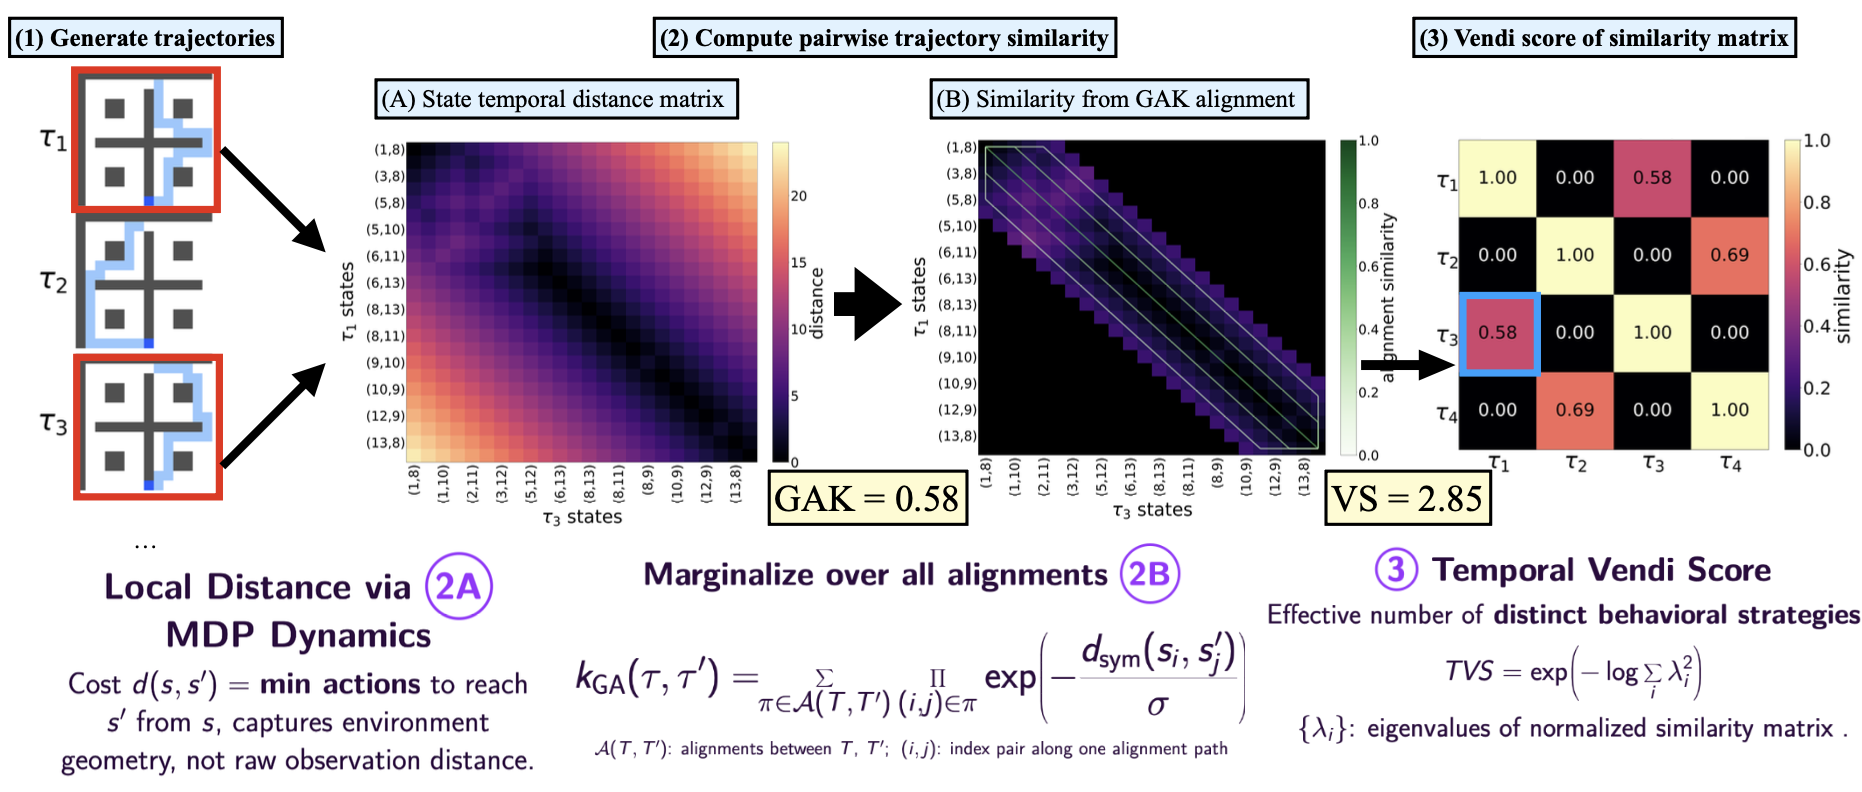
\includegraphics[width=1.0\linewidth]{figures/method_v3.pdf}
    \end{block}
    \endgroup
  \end{column}
  \separatorcolumn
\end{columns}

\vspace{1cm}




% ====================
% Row 4: Experiments (left, wide) + Descriptions (right, narrow)
% ====================
\begin{columns}[t]
  \separatorcolumn

  % ---- LEFT: 3 experiment plots stacked ----
  \begin{column}{0.7\paperwidth}
    \begin{block}{Experiments \& Key Results}

     % --- Continuous Control ---
      \raggedright{\Large\bfseries\textcolor{blockheader}{Continuous Control}}\\[0.15em]
      \centering
      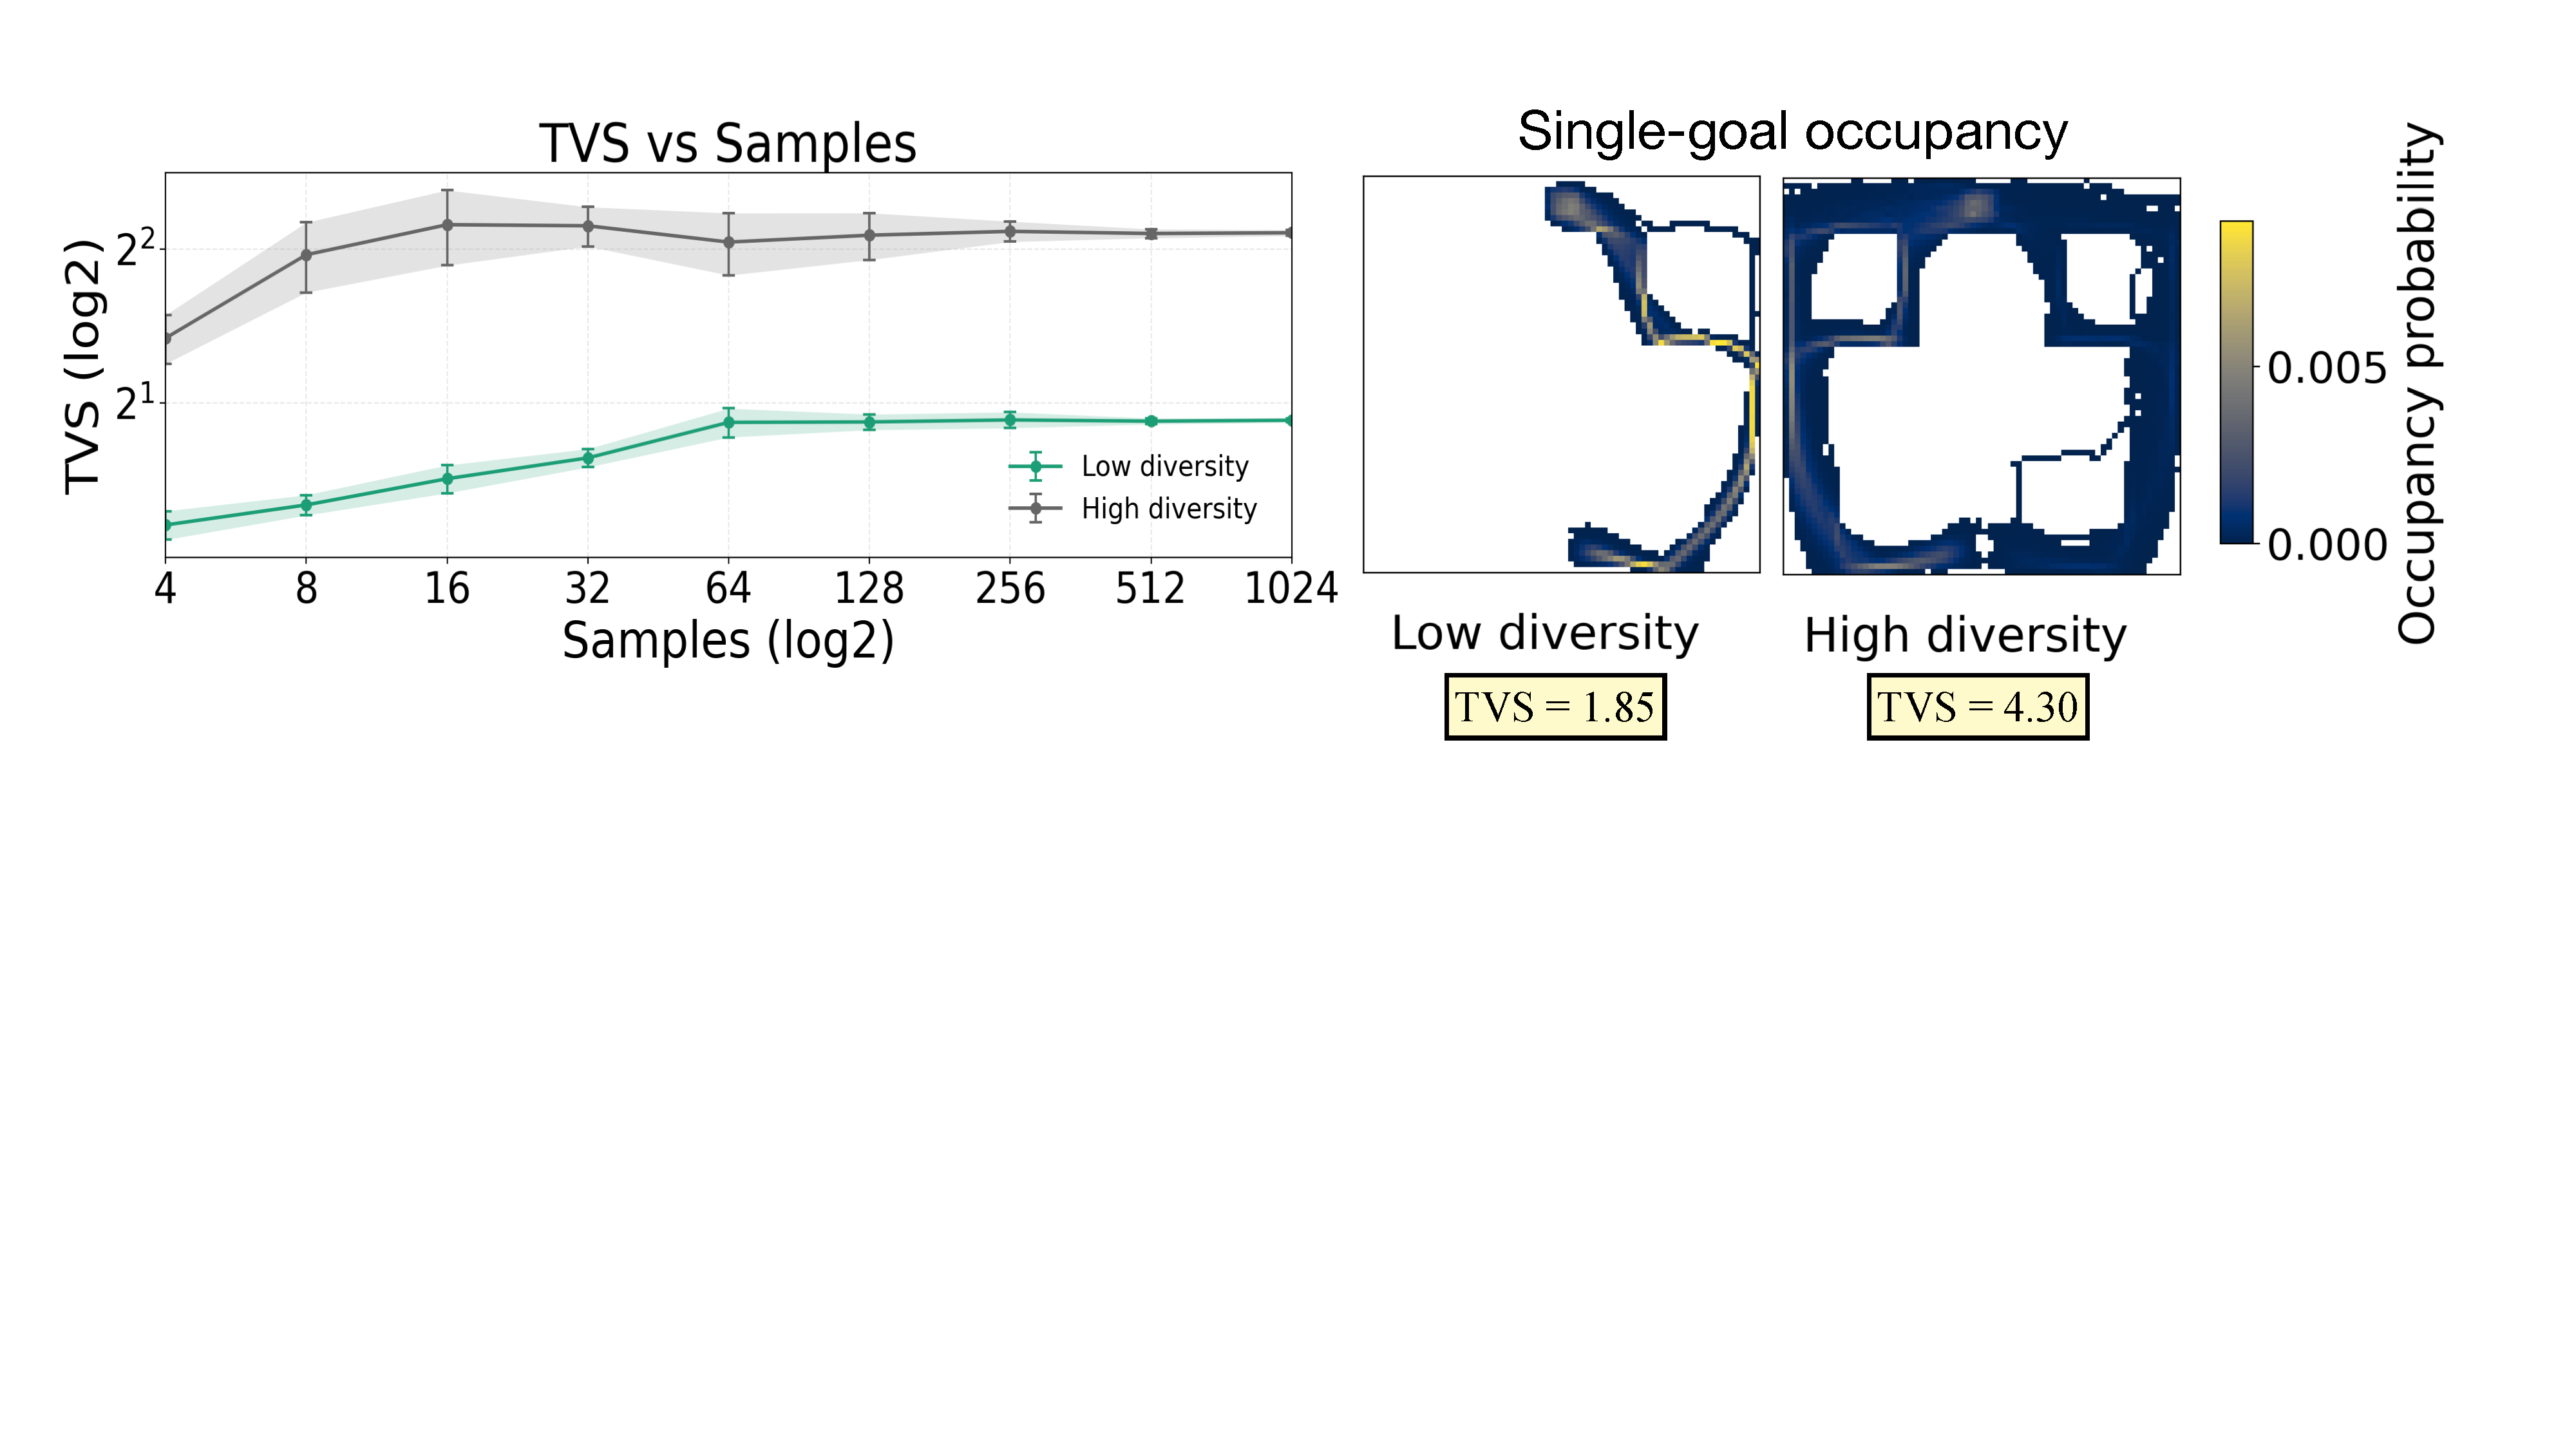
\includegraphics[width=\linewidth]{figures/continuous.pdf}
      
       \vspace{0.3cm}
       

      % --- Superiority Over Baselines ---
      \raggedright{\Large\bfseries\textcolor{blockheader}{Superiority Over Baselines}}\\[0.15em]
      \hspace*{-1.5cm}
      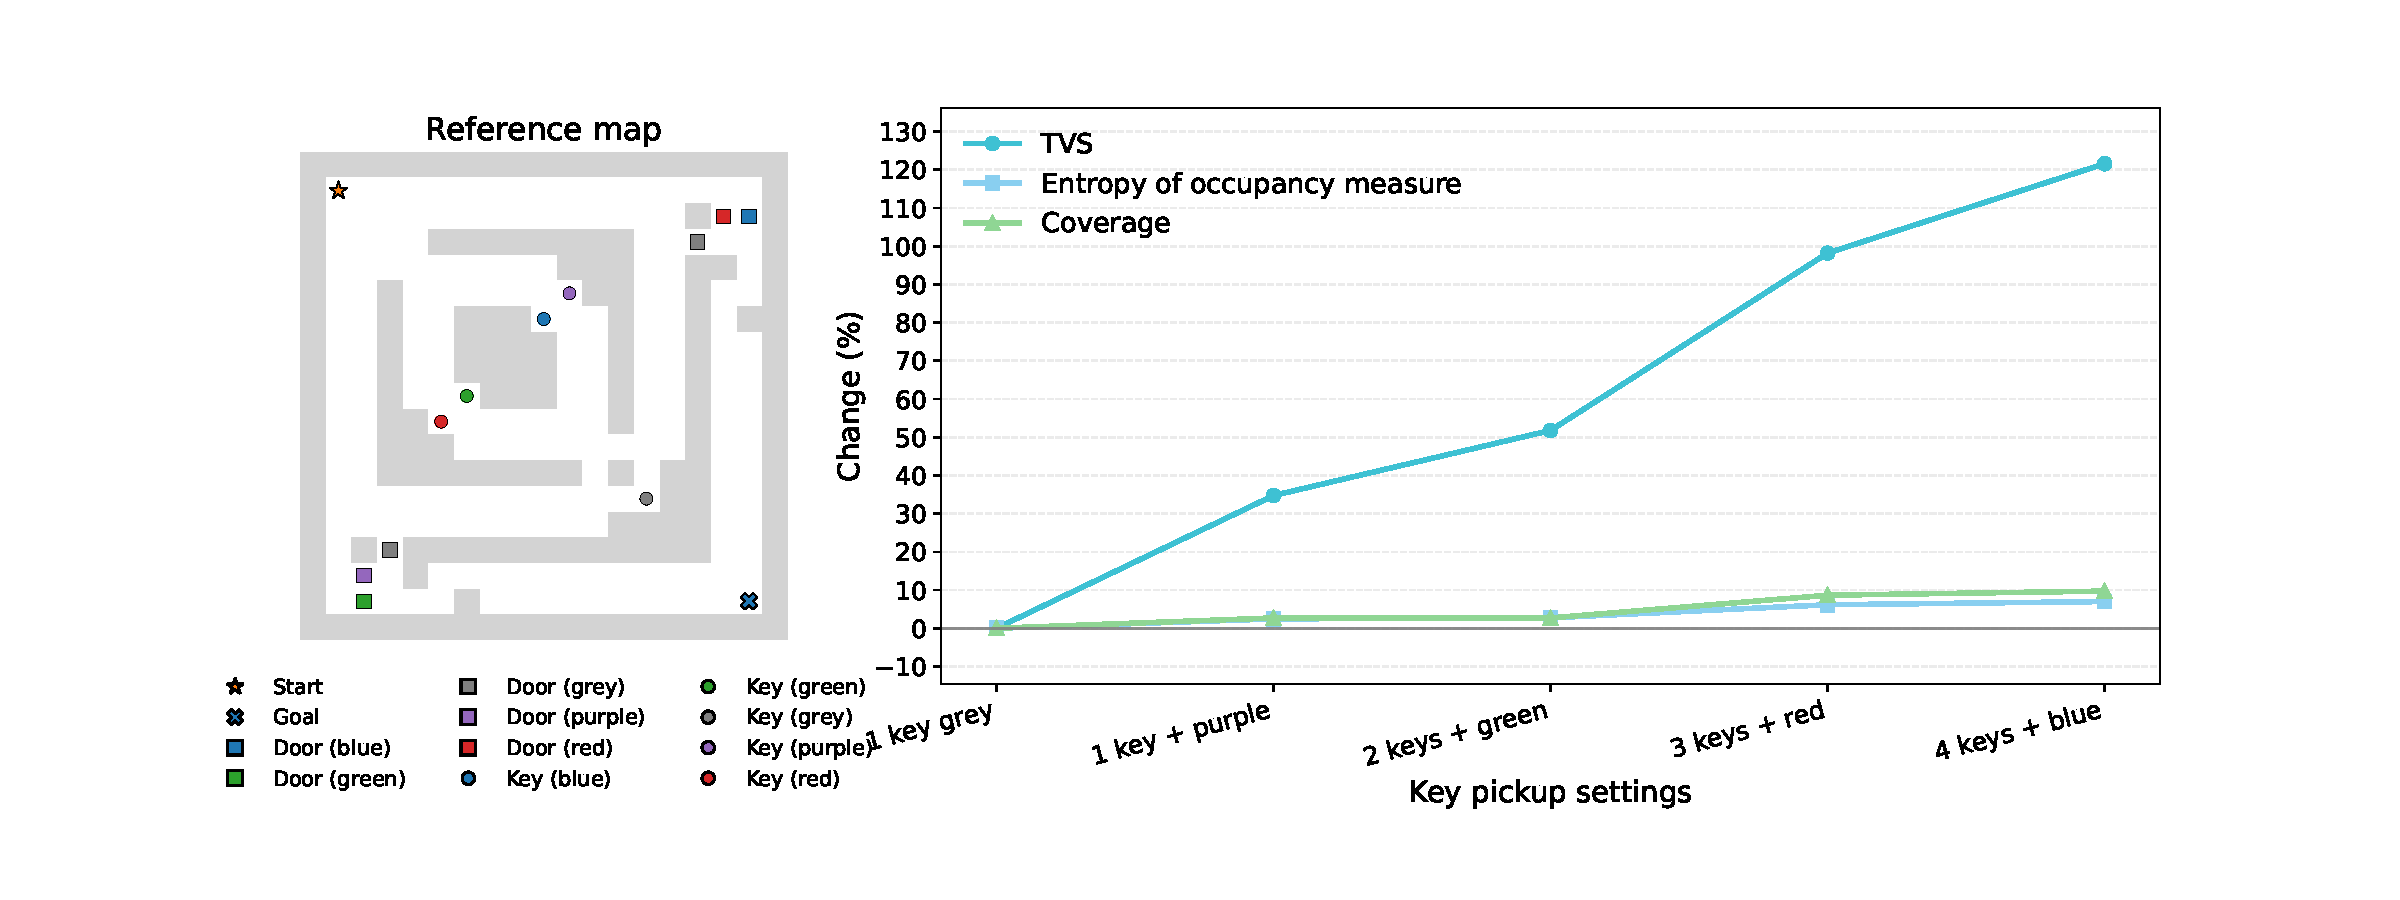
\includegraphics[width=1.0\linewidth]{figures/key.pdf}



      
      \end{block}
  \end{column}

  \separatorcolumn

  % ---- RIGHT: Experiment Descriptions + References ----
  \begin{column}{0.2\paperwidth}

    \begin{block}{Continuous Control}
      \footnotesize
		\LARGE
		
		
      \metric{} scales to continuous point-maze environments using learned quasimetric distances.
          \end{block}
          
              \vspace{0.3cm}

          
    \begin{block}{Superiority Over Baselines.}
      \footnotesize
		\LARGE
		As the agent learns to use 1–5 keys in a maze, state coverage and occupancy entropy stay nearly flat. The diversity is temporal, not spatial. \metric{} correctly captures this sequential structure and increases steadily with each new strategy.



	 \end{block}
% ====================
% Row 5: References
% ====================
\begingroup
\setbeamercolor{block title}{fg=white, bg=black}
\setbeamercolor{block body}{fg=darktext, bg=white}
\begin{block}{References}
    \footnotesize
    \begin{thebibliography}{9}
        \setbeamertemplate{bibliography item}[text] % Use numbers instead of icons
        
        \bibitem{cuturi2007kernel} 
        M.~Cuturi et al. \textit{A kernel for time series based on global alignments.} ICASSP, 2007.

        \bibitem{eysenbach2018diversityneedlearningskills} 
        B.~Eysenbach et al. \textit{Diversity is all you need: Learning skills without a reward function.} ICLR, 2019.

        \bibitem{friedman2023vendi} 
        D.~Friedman \& A.B.~Dieng. \textit{The Vendi Score: A diversity evaluation metric for ML.} 2023.
    \end{thebibliography}
\end{block}
\endgroup

  \end{column}

  \separatorcolumn
\end{columns}

\end{frame}
\end{document}
